\documentclass[11pt,a4paper]{article}

\usepackage[utf8]{inputenc}
\usepackage[T1]{fontenc}
\usepackage{amsmath}
\usepackage{booktabs}
\usepackage{geometry}
\usepackage{graphicx}
\usepackage{hyperref}
\usepackage{xcolor}

\geometry{margin=2.4cm}

\hypersetup{
    colorlinks=true,
    linkcolor=blue!60!black,
    urlcolor=blue!60!black
}

\title{Resultados finais: Laplaciano vs. KMeans direto}
\author{Trabalho de Teoria Espectral}
\date{\today}

\begin{document}

\maketitle

\section{Configuração experimental}

Foram avaliados três conjuntos de embeddings:

\begin{enumerate}
    \item \textbf{DINOv2 CUB50}: primeiras 50 classes do CUB-200-2011, totalizando 2889 imagens.
    \item \textbf{DINOv2 Flowers}: Oxford Flowers com 17 classes e 80 imagens por classe.
    \item \textbf{AlexNet Flowers}: Oxford Flowers usando embeddings extraídos da AlexNet pré-treinada.
\end{enumerate}

Para o método com grafo, usamos a pipeline:
\[
\text{embedding} \rightarrow \text{ranking KNN} \rightarrow W \rightarrow
L = I - D^{-1/2}WD^{-1/2} \rightarrow \text{autovetores} \rightarrow \text{KMeans}.
\]

O valor usado para o grafo KNN foi:
\[
K=20.
\]

Para a ablação, também rodamos KMeans diretamente sobre as matrizes de embeddings,
sem construir grafo e sem usar autovetores do Laplaciano.

\section{Métricas}

Como os índices produzidos pelo KMeans são arbitrários, antes de calcular a
acurácia fazemos o melhor pareamento cluster-classe com o algoritmo Húngaro.
Nesta tabela, ``Acc.'' significa essa acurácia após pareamento ótimo.

\begin{center}
\begin{tabular}{llccc}
\toprule
Experimento & Método & Acc. & ARI & NMI\\
\midrule
DINOv2 CUB50 & Laplaciano & 0.7480 & 0.6835 & 0.8842\\
DINOv2 CUB50 & KMeans direto & 0.7847 & 0.7196 & 0.8803\\
\midrule
DINOv2 Flowers & Laplaciano & 1.0000 & 1.0000 & 1.0000\\
DINOv2 Flowers & KMeans direto & 0.9963 & 0.9921 & 0.9930\\
\midrule
AlexNet Flowers & Laplaciano & 0.6449 & 0.5262 & 0.7209\\
AlexNet Flowers & KMeans direto & 0.6404 & 0.4749 & 0.6792\\
\bottomrule
\end{tabular}
\end{center}

\section{Leitura dos resultados}

No Flowers com DINOv2, os dois métodos são praticamente perfeitos. O Laplaciano
atinge 100\% nas três métricas, enquanto o KMeans direto fica muito próximo.
Isso indica que os embeddings do DINOv2 já separam muito bem as classes desse
dataset.

No CUB50 com DINOv2, o KMeans direto obteve acurácia e ARI maiores, enquanto o
Laplaciano ficou levemente melhor em NMI. Isso sugere que, para esse subconjunto,
o espaço DINOv2 direto já contém uma estrutura de classes forte; o grafo KNN não
melhorou a separação medida por acurácia.

No Flowers com AlexNet, o Laplaciano teve pequena vantagem sobre o KMeans direto:
a acurácia subiu de 0.6404 para 0.6449, o ARI de 0.4749 para 0.5262 e o NMI de
0.6792 para 0.7209. Aqui o grafo ajudou mais, provavelmente porque os embeddings
da AlexNet são menos alinhados com as classes do que os embeddings do DINOv2.

\section{Arquivos gerados}

Os resultados numéricos da ablação foram salvos em:

\begin{itemize}
    \item \texttt{DataSets/Laplacian/FinalAblation/metrics.csv}
    \item \texttt{DataSets/Laplacian/FinalAblation/metrics.json}
\end{itemize}

Os arrays do KMeans direto foram salvos em:

\begin{itemize}
    \item \texttt{DataSets/Laplacian/FinalAblation/KMeansOnly/}
\end{itemize}

Os resultados do Laplaciano com AlexNet foram salvos separadamente em:

\begin{itemize}
    \item \texttt{DataSets/Laplacian/AlexNet/}
\end{itemize}

\section{Figuras do AlexNet}

\begin{figure}[h]
    \centering
    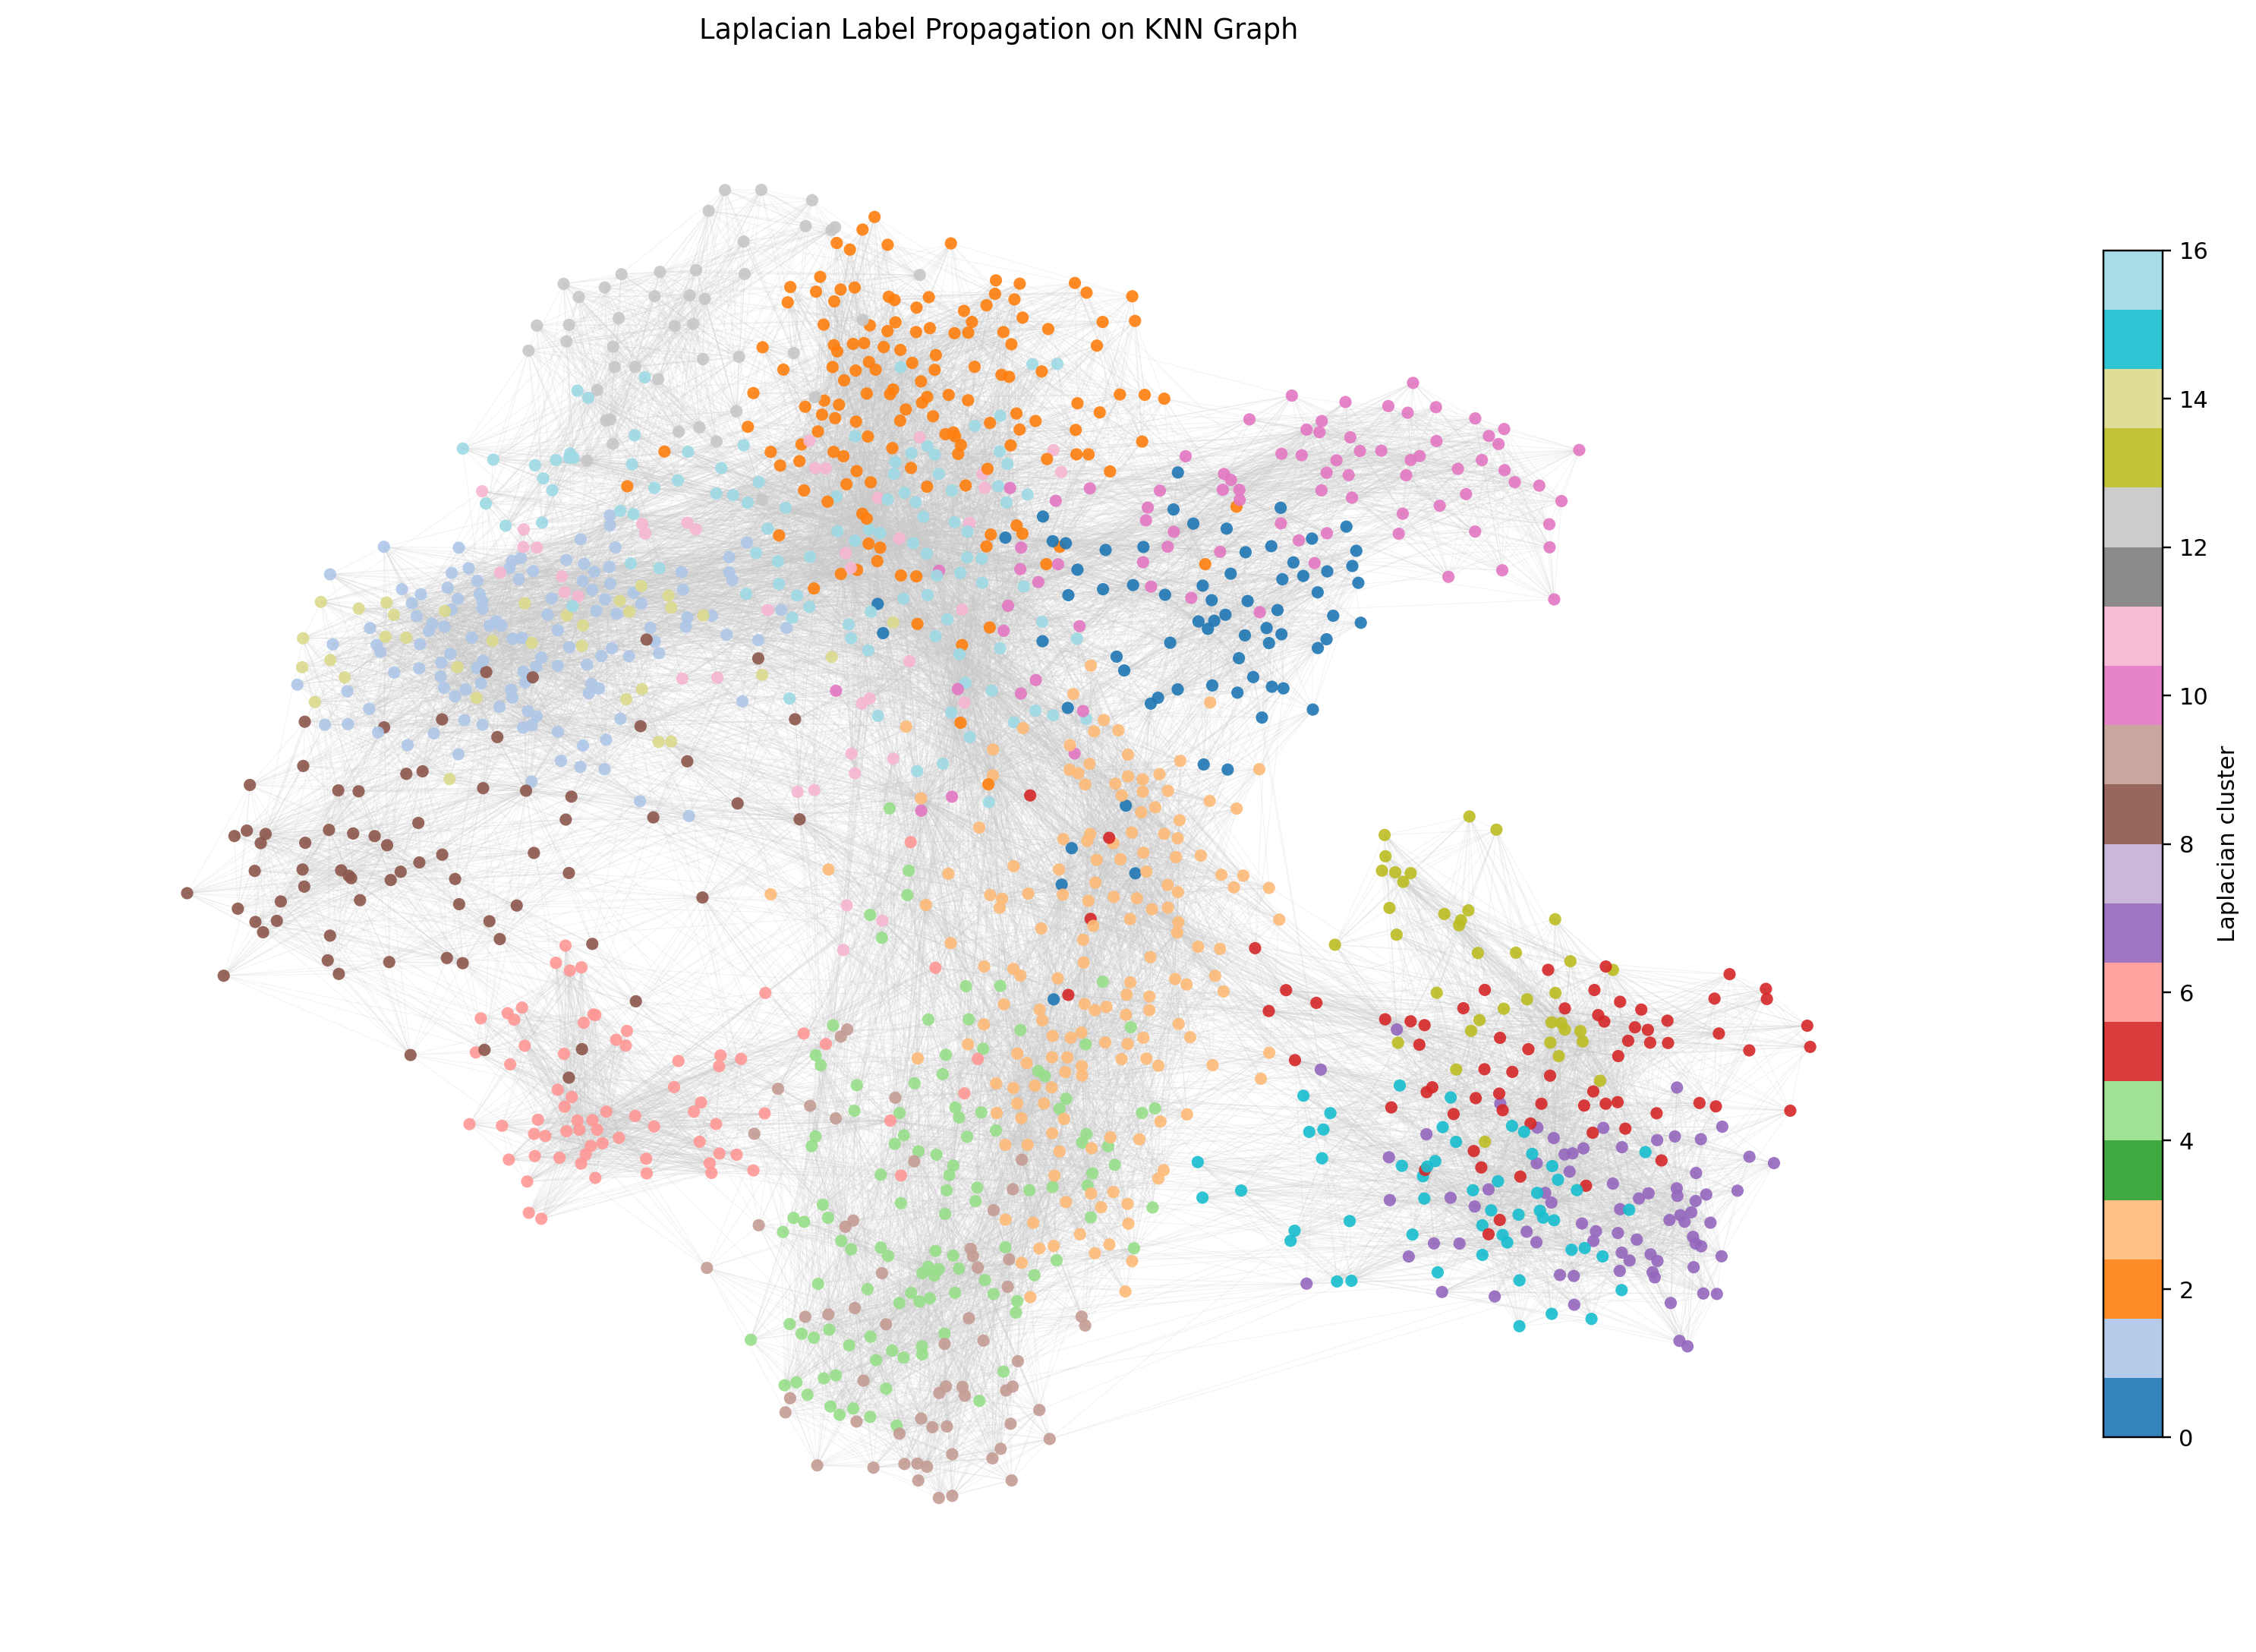
\includegraphics[width=0.92\linewidth]{../DataSets/Laplacian/AlexNet/AlexNet_Flowers_laplacian_label_propagation_k20_c17.png}
    \caption{Grafo KNN do AlexNet Flowers colorido pelos clusters espectrais.}
\end{figure}

\begin{figure}[h]
    \centering
    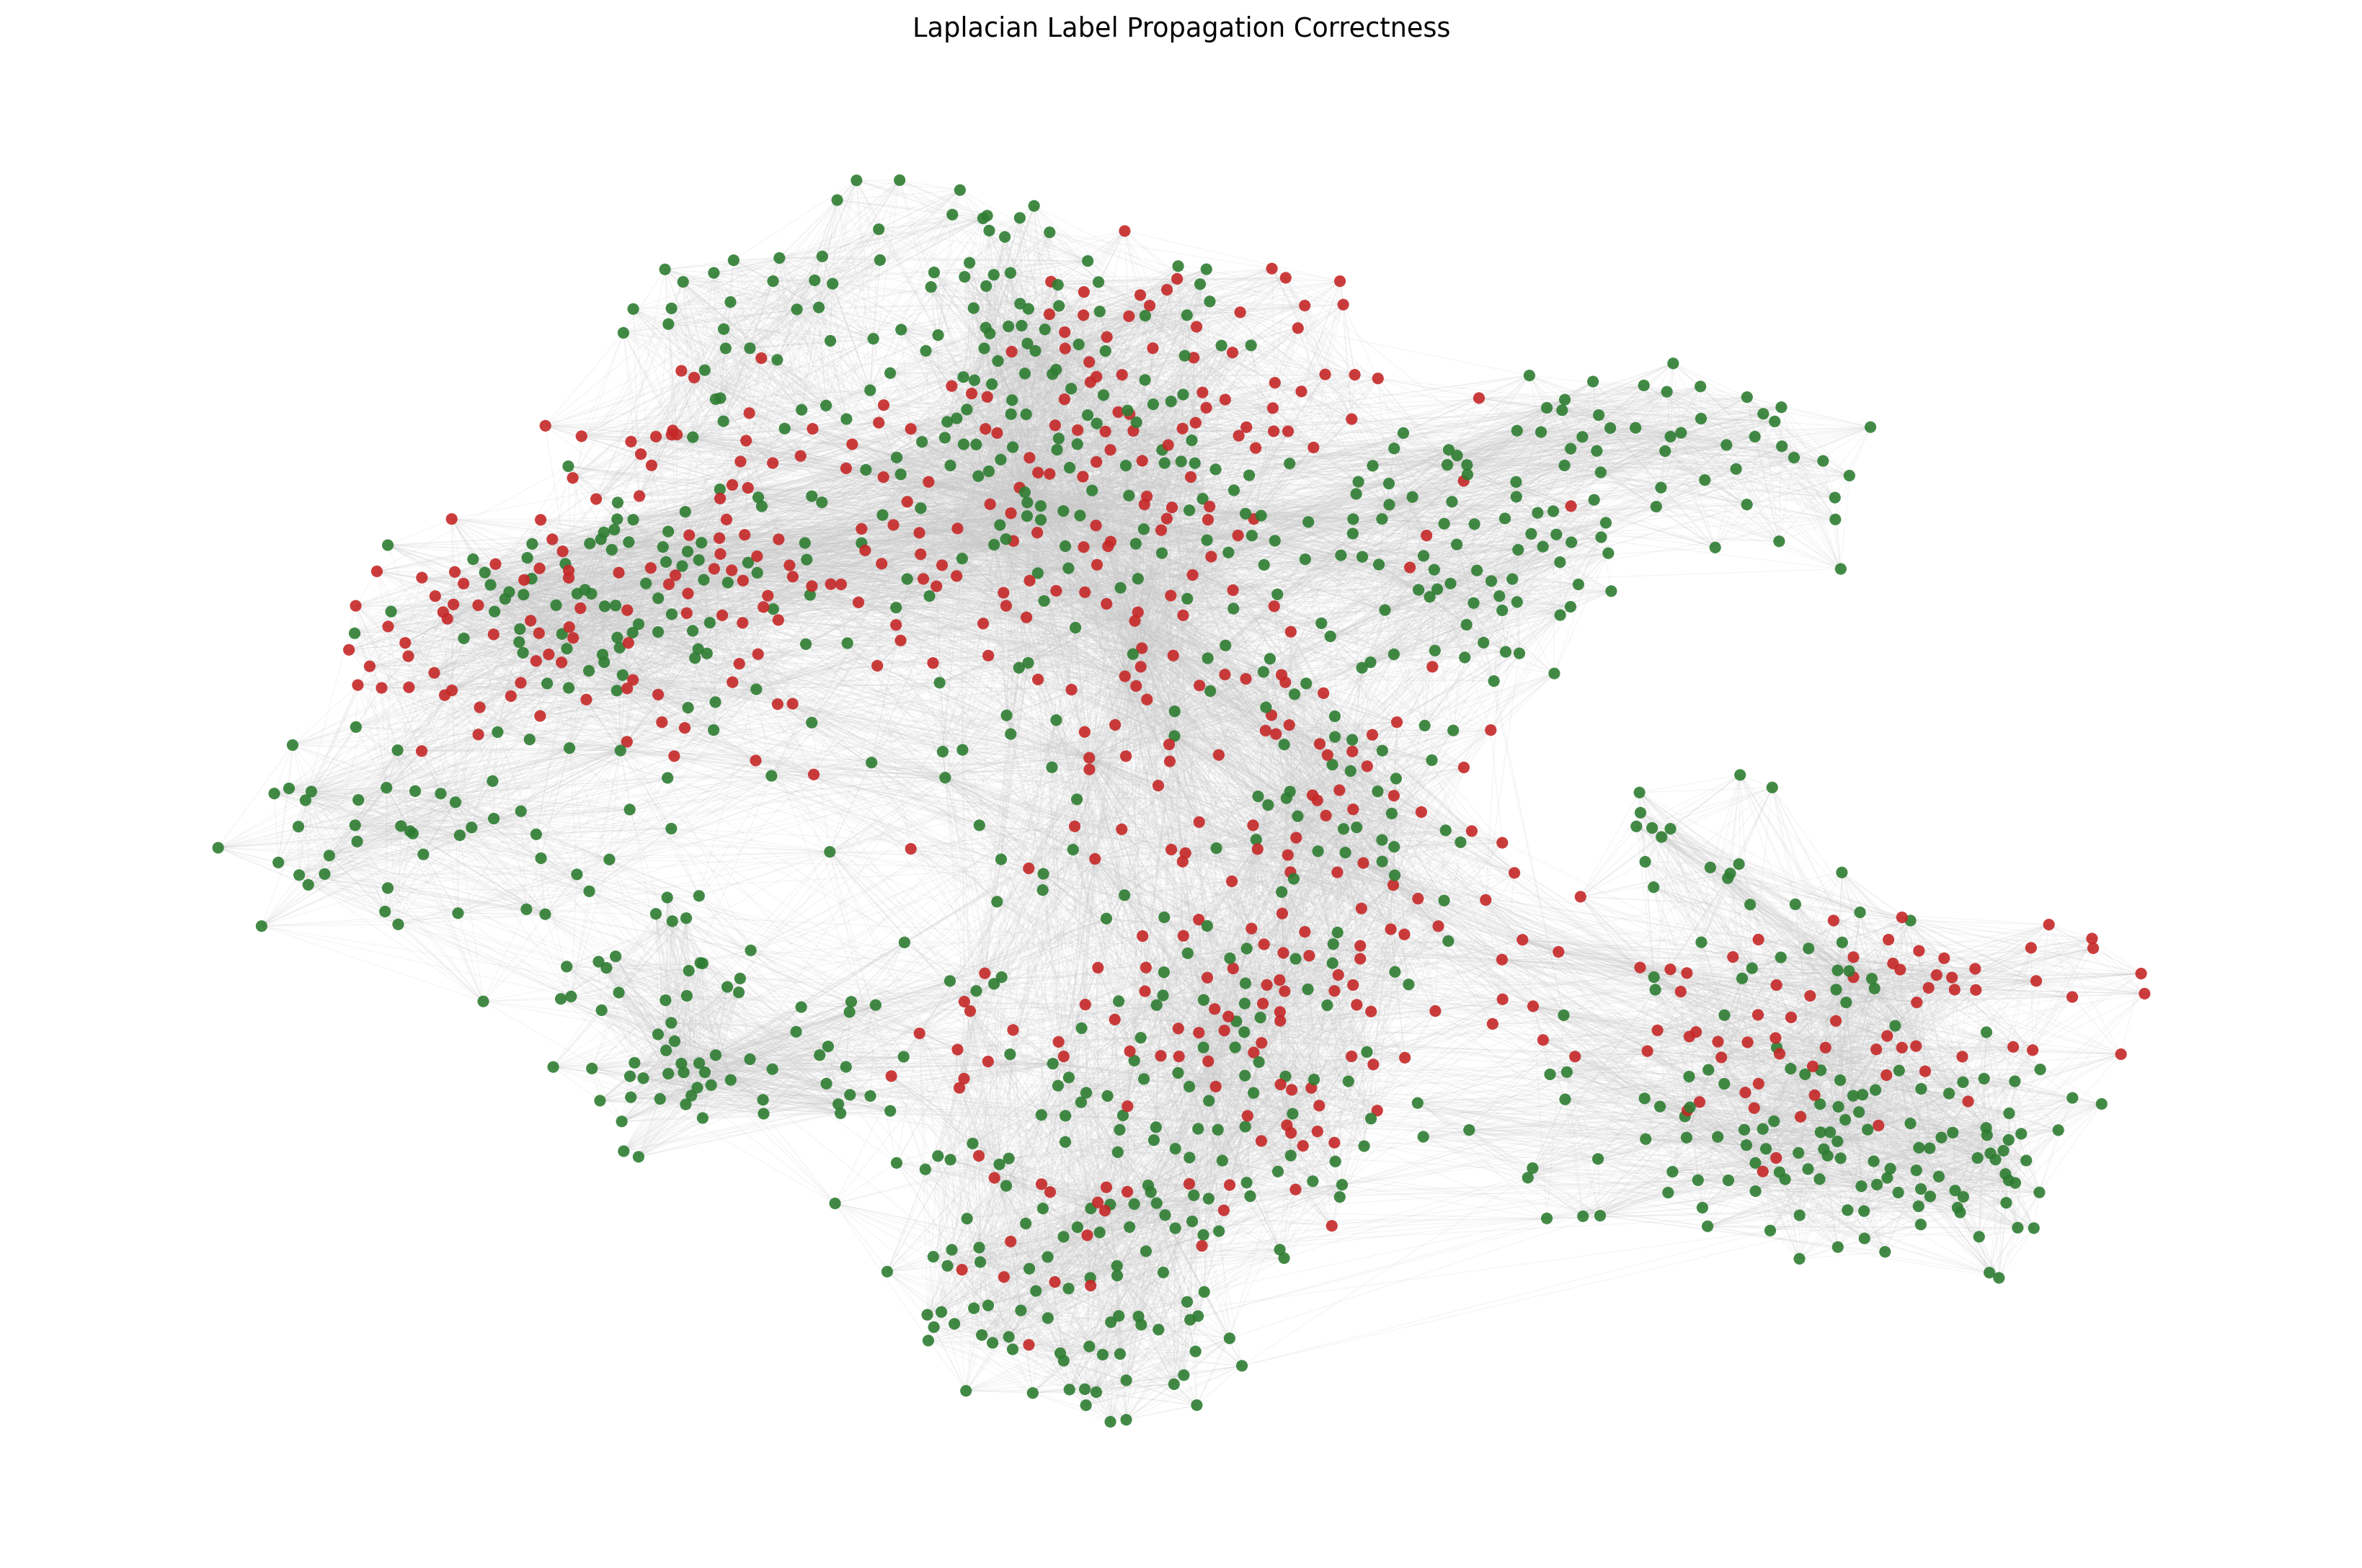
\includegraphics[width=0.92\linewidth]{../DataSets/Laplacian/AlexNet/AlexNet_Flowers_laplacian_label_propagation_k20_c17_correctness.png}
    \caption{Grafo KNN do AlexNet Flowers colorido por acerto/erro após pareamento ótimo.}
\end{figure}

\begin{figure}[h]
    \centering
    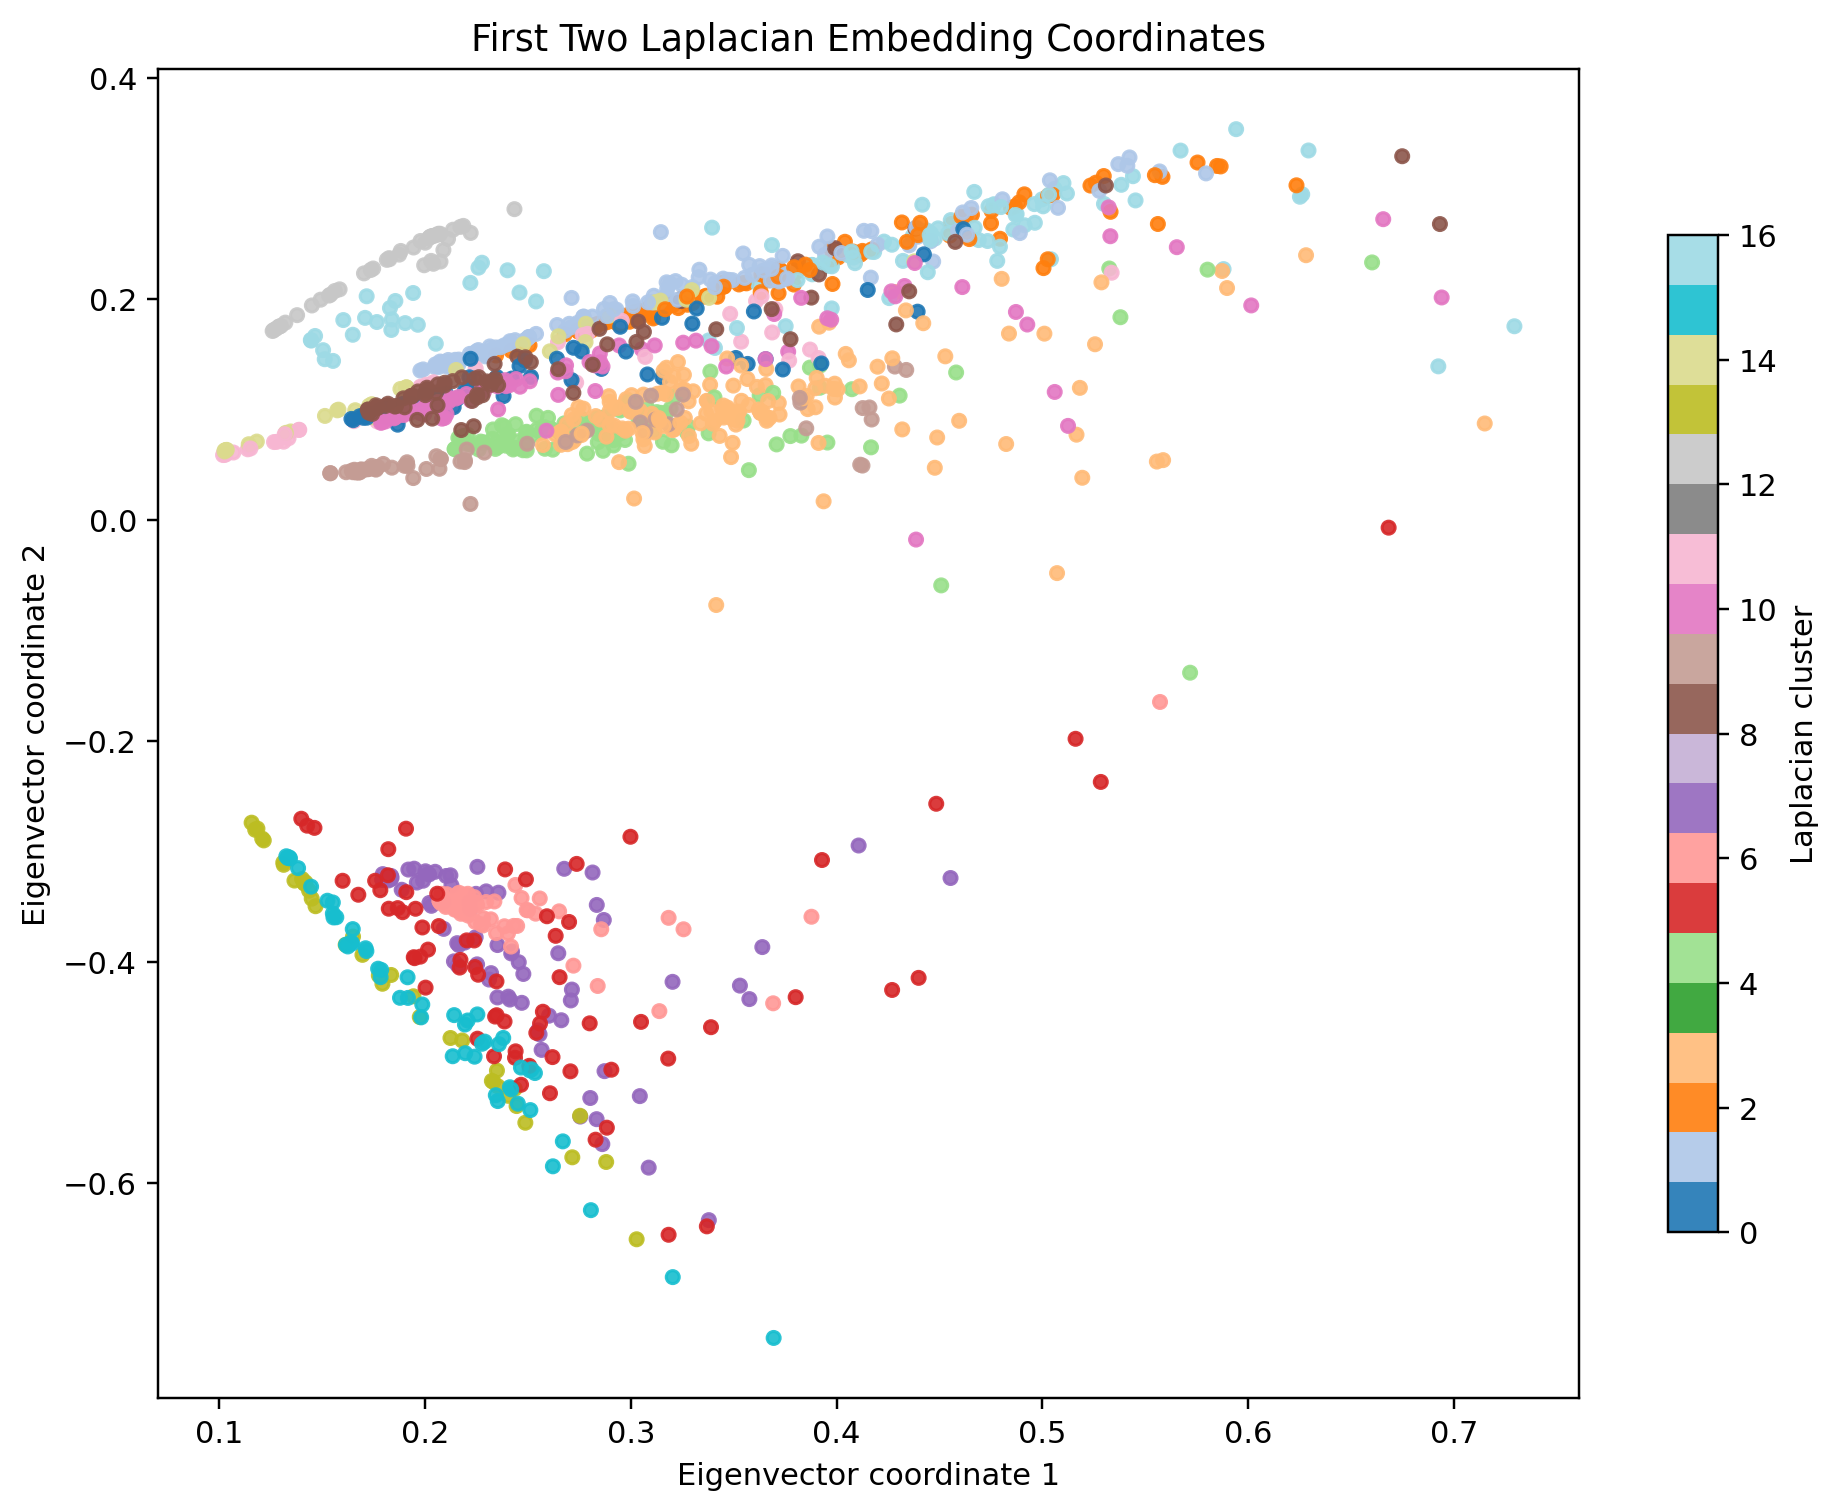
\includegraphics[width=0.72\linewidth]{../DataSets/Laplacian/AlexNet/AlexNet_Flowers_laplacian_label_propagation_k20_c17_embedding.png}
    \caption{Duas primeiras coordenadas do embedding laplaciano para AlexNet Flowers.}
\end{figure}

\section{Conclusão}

A comparação mostra que o ganho do Laplaciano depende da qualidade e da geometria
do embedding inicial. Com DINOv2 em Flowers, as classes já estão quase
perfeitamente separadas. Com AlexNet em Flowers, o Laplaciano melhora as métricas
em relação ao KMeans direto, indicando que a estrutura de vizinhança do grafo
ajuda quando o embedding inicial é menos discriminativo.

\end{document}
